% Slides for talk on hydrogen fuel cells
% given in the department on October 27, 2003.
% 
% The original slides were in Prosper.  This file contains the
% translation of the original slides to Beamer.
% 
% Rouben Rostamian <rostamian@umbc.edu>
% August 31, 2004

\documentclass[10pt]{beamer}
\usepackage{CJKutf8} %支持中文
\usepackage{pdfpages}
\usetheme{umbc4}

\useinnertheme{umbcboxes}
\setbeamercolor{umbcboxes}{bg=violet!12,fg=black}

\usepackage{rotating} % for defining \schwa
\newcommand{\schwa}{\raisebox{1ex}{\begin{turn}{180}e\end{turn}}}

\newcommand{\arcsinh}{\mathop\mathrm{arcsinh}\nolimits}
\newcommand{\arccosh}{\mathop\mathrm{arccosh}\nolimits}
\newcommand{\Pu}{P_{\mathrm{amb}}}

% \subtitle{Modeling and Computations}
\subtitle{A opensource dict client of youdao for linux}
\author[NetEase]{Bjzhangxin}
\title{Openyoudao}
\date{September 10, 2013}

\begin{document}
\begin{CJK*}{UTF8}{song} %中文支持
\CJKfamily{gkai} %中文支持
%----------- titlepage ----------------------------------------------%
\begin{frame}[plain]
  \titlepage
\end{frame}

%----------- slide --------------------------------------------------%
\begin{frame}
  \frametitle{\Large{History 2012--04--16 A boring Day!!!}}

\begin{center} 
  
\includegraphics[width=0.4\textwidth]{pic1.jpg}
\end{center}
\medskip
\quad
\qquad

I am linuxer, Reading paper just so boring, I can't bear it any more!!!
\end{frame}
%----------- slide --------------------------------------------------%
\begin{frame}
  \frametitle{\Large{How to complete it?}}
\begin{itemize}
 \LARGE{\item How to take the word that i want?
  \item How to translate it?
  \item How to show it?}
\end{itemize}
\end{frame}
%----------- slide --------------------------------------------------%
\begin{frame}
  \frametitle{\Large{常用开源取词技术}}
\LARGE\begin{itemize}
 {\item \href{http://nullege.com/codes/show/src@p@y@python-xlib-HEAD@trunk@examples@record_demo.py/86/Xlib.display.Display.record_create_context}{剪切板取词}
  \item \href{https://code.google.com/p/tesseract-ocr/}{OCR取词}
  \item \href{http://www.athoughtabroad.com/2013/05/22/using-google-s-speech-recognition-web-service-with-python}{语音取词}}
\end{itemize}
\end{frame}
%----------- slide --------------------------------------------------%
\begin{frame}
  \frametitle{取词原理}
\begin{center} 
  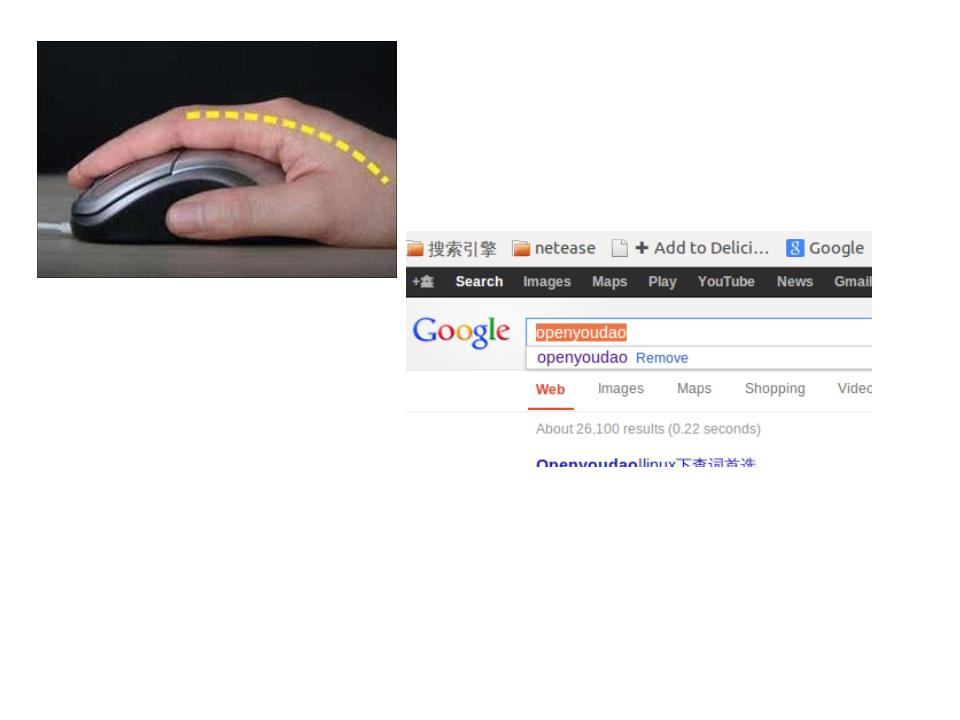
\includegraphics[width=1.1\textwidth]{shijian.jpg}
\end{center}
\end{frame}

%----------- slide --------------------------------------------------%
\begin{frame}
   \frametitle{剪切板取词}
if event.type == X.ButtonRelease: \\
    pipe = os.popen("xclip -o") \\
    text = pipe.readline() \\
    pipe.readlines() \\
    pipe.close() \\
    print "您选取的是: ", text \\
\end{frame}

%----------- slide --------------------------------------------------%
\begin{frame}
  \frametitle{\Large{常用开源取词技术}}
\LARGE\begin{itemize}
 {\item \href{http://nullege.com/codes/show/src@p@y@python-xlib-HEAD@trunk@examples@record_demo.py/86/Xlib.display.Display.record_create_context}{剪切板取词}
  \item \href{https://code.google.com/p/tesseract-ocr/}{OCR取词}
  \item \href{http://www.athoughtabroad.com/2013/05/22/using-google-s-speech-recognition-web-service-with-python}{语音取词}}
\end{itemize}
\end{frame}

%----------- slide --------------------------------------------------%
\begin{frame}
   \frametitle{OCR取词}
   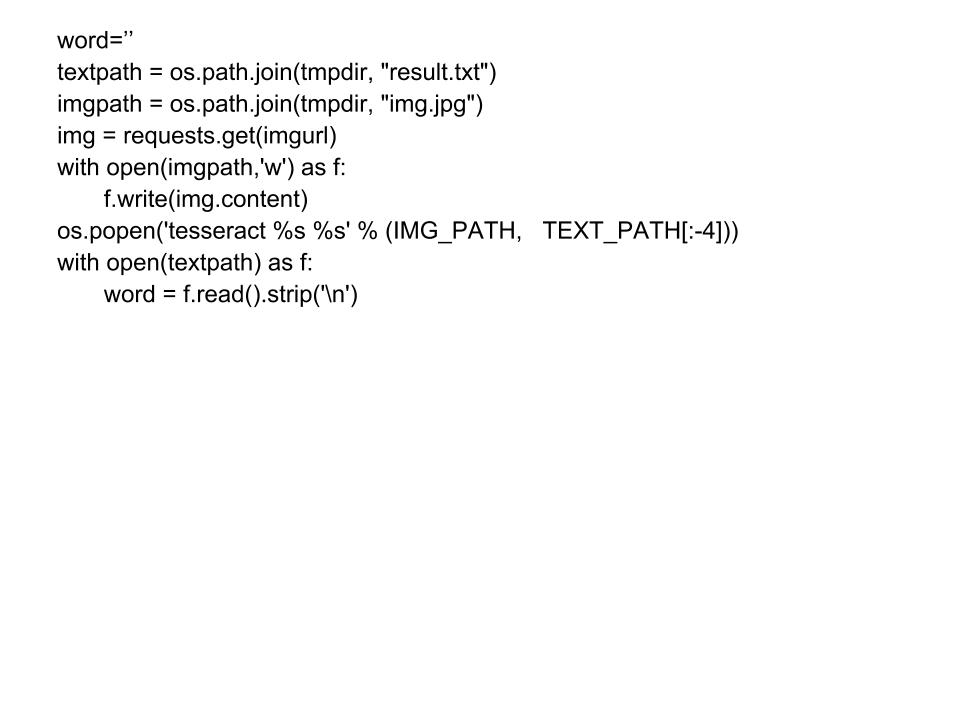
\includegraphics[width=1.2\textwidth]{ocr.jpg}
   %imgpath = os.path.join(tmpdir, "img.jpg") \\
   %img = requests.get(imgurl) \\
   %with open(umgpath,'w') as f: \\
   %f.write(img.content) \\
   %os.popen('tesseract %s %s' % (IMG_PATH, TEXT_PATH[:-4])) \\ 
   %with open(textpath) as f: \\
   %word = f.read().strip('n') \\
\end{frame}

%----------- slide --------------------------------------------------%
\begin{frame}
  \frametitle{\Large{常用开源取词技术}}
\LARGE\begin{itemize}
 {\item \href{http://nullege.com/codes/show/src@p@y@python-xlib-HEAD@trunk@examples@record_demo.py/86/Xlib.display.Display.record_create_context}{剪切板取词}
  \item \href{https://code.google.com/p/tesseract-ocr/}{OCR取词}
  \item \href{http://www.athoughtabroad.com/2013/05/22/using-google-s-speech-recognition-web-service-with-python}{语音取词}}
\end{itemize}
\end{frame}

%----------- slide --------------------------------------------------%
\begin{frame}
  \frametitle{\Large{如何在线翻译}}
\LARGE\begin{itemize}
 {\item 目前流行的在线翻译网站
  \item 译文下载
  \item 页面重构}
\end{itemize}
\end{frame}

%----------- slide --------------------------------------------------%
%\begin{frame}
%  \frametitle{\Large{流行的在线翻译网站}}
%\LARGE\begin{itemize}
%  {%\item \href{http://dict.youdao.com/search?q=}{有道字典}
%   %\item \href{http://www.iciba.com/}{爱词霸}
%   \item \href{http://translate.google.cn/#en/zh-CN/}{谷歌翻译}}
%   }
%\end{itemize}
%\end{frame}

%----------- slide --------------------------------------------------%
\begin{frame}
  \frametitle{\Large{流行的在线翻译网站}}
\LARGE\begin{itemize}
 {\item \href{http://dict.youdao.com/search?q=}{有道字典}
  \item \href{http://www.iciba.com/}{爱词霸}
  \item \href{http://translate.google.cn/\#en/zh-CN/}{谷歌翻译}}
\end{itemize}
\end{frame}

%----------- slide --------------------------------------------------%
\begin{frame}
  \frametitle{\Large{如何在线翻译}}
\LARGE\begin{itemize}
 {\item 目前流行的在线翻译网站
  \item 译文下载
  \item 页面重构}
\end{itemize}
\end{frame}


%----------- slide --------------------------------------------------%
\begin{frame}
   \frametitle{译文下载}
   curl -s -o origin.html http://dict.youdao.com/search?q=youdao
\end{frame}

%----------- slide --------------------------------------------------%
\begin{frame}
  \frametitle{\Large{如何在线翻译}}
\LARGE\begin{itemize}
 {\item 目前流行的在线翻译网站
  \item 译文下载
  \item 页面重构}
\end{itemize}
\end{frame}

%----------- slide --------------------------------------------------%
\begin{frame}
   \frametitle{页面重构}
\LARGE\begin{itemize}
 {\item 提取正文
  \item 布局文件本地化
  \item 修复部分js
 }
\end{itemize}
\end{frame}
%----------- slide --------------------------------------------------%
\begin{frame}
   \frametitle{主流浏览器内核}
\Large\begin{itemize}
 {\item Webkit
  \item Gecko(Firefox内核)
  \item Presto(Opera前内核)
  \item Blink(Chrome的未来内核)
  \item Trident(IE内核)
 }
\end{itemize}
\end{frame}

%----------- slide --------------------------------------------------%
\begin{frame}
   \frametitle{结果显示}
   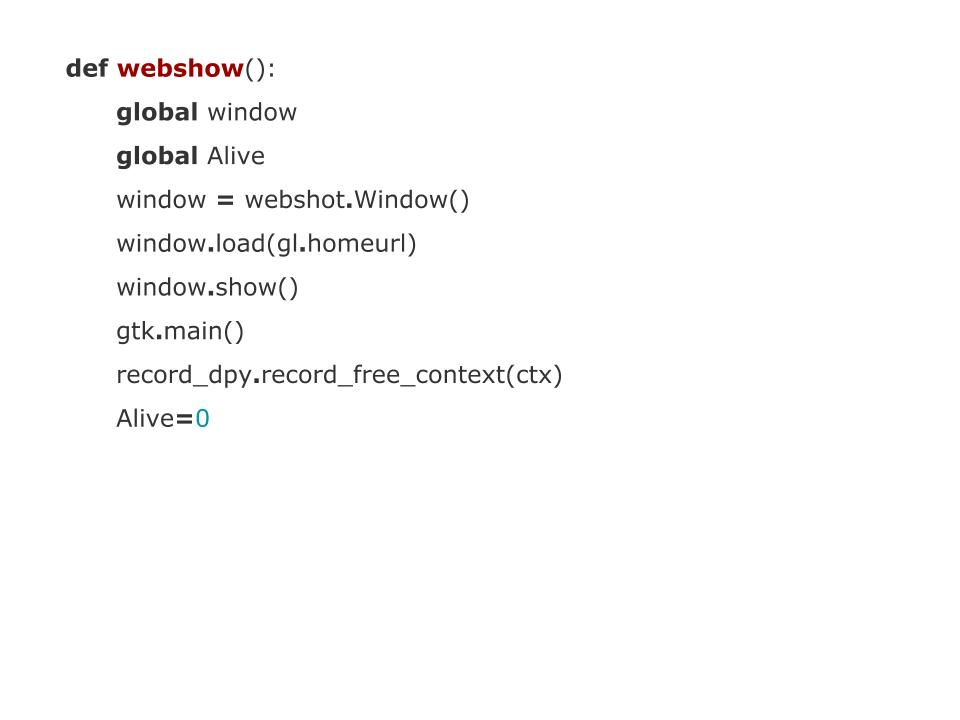
\includegraphics[width=1.0\textwidth]{result.jpg}
\end{frame}

%----------- slide  --------------------------------------------------%
\begin{frame}
  \frametitle{\Large{What problems exist ?}}
\begin{itemize}
{ 
  \item 如何提取翻译正文(有道广告不错,就是把译文挡住了,囧~) 
  \item 添加其它字典(侧边栏,ok?)
  \item 如何防止用户刷屏(管道原来可以这样用~~~)
  \item 离线字库(还是先人肉吧)
  \item 如何退出程序(玩一把汇编~软中断) 
  \item 刷新取词结果
}
\end{itemize}
\end{frame}

%----------- slide --------------------------------------------------%
\begin{frame}
   \frametitle{程序设计原则}
\Large\begin{itemize}
 {\item 界面上永远不许有按钮
  \item 主程序中既是测试程序,不许有功能模块
  \item 所有功能模块保持最大化的独立,尤其是界面和程序不许纠缠
 }
\end{itemize}
\end{frame}
%----------- slide --------------------------------------------------%
\begin{frame}
  \frametitle{How to Join Us?}

\begin{itemize}
\large{
  \item homepage: http://openyoudao.org/
  \item github:git@github.com:justzx2011/openyoudao.git
  \item mail: justzx2011@gmail.com  @justzx
  \item twitter: @openyoudao
  \item maillist: openyoudao@googlegroups.com
}
  
\end{itemize}

\end{frame}

%----------- slide --------------------------------------------------%
\begin{frame}
  \frametitle{Thanks}
\begin{center} 
  
\includegraphics[width=0.6\textwidth]{thanks.png}
\end{center}
\end{frame}

%----------- slide --------------------------------------------------% 
\end{CJK*}
\end{document}
